\section{Guided Backpropagation}\label{section:gbp}

Guided Backpropagation (GBP) \cite{springenberg2014striving} is an approach designed by Springenberg et al., relying on the ideas of \textit{Deconvolution} (Section \ref{section:deconvolution}) and \textit{Saliency} (Section \ref{section:saliency}). Authors argue that the approach taken by Simonyan et al. \cite{simonyan2014deep} has an issue with the flow of negative gradients, which decreases the accuracy of the higher layers we are trying to visualize. Their idea is to combine two approaches and add a "guide" to the \textit{Saliency} with the help of deconvolution.

\vspace{\baselineskip}

To achieve that, we have to focus on the \textit{ReLU} activation function in the CNN. When computing values at the \textit{Rectification} component of the \textit{deconvnet}, we are masking all non-positive values with the \textit{ReLU}. In that layer, the computed values are calculated only base on the top signal (reconstruction from the upper layer), and the input is ignored. On the other hand, in the \textit{Saliency} method, we are focusing on the gradient values computed base on the input image. If we take deconvnet masking of the \textit{Rectification} layer and apply it on the gradient values of the \textit{Saliency} method, we could remove noise caused by the negative gradient values. This noise removal is the reason why the method has the prefix "guided". Deconvolution guides backpropagation values of the \textit{Saliency} method to produce sharper images (Fig. \ref{fig:gbp-gbp-attribution}).

\begin{figure}[h]
  \centering
 \begin{subfigure}{.2\textwidth}
    \centering
    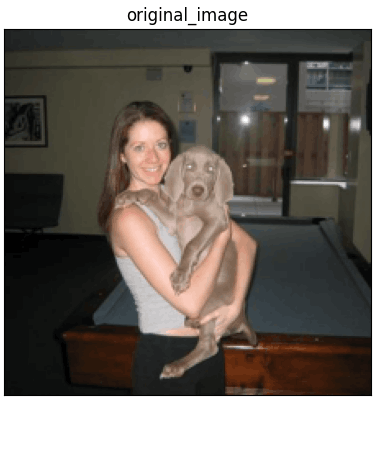
\includegraphics[width=\textwidth]{methods/images/Weimaraner-image.png}
    \caption{Original image}\label{fig:gbp-weimaraner}
\end{subfigure}
 \begin{subfigure}{.25\textwidth}
    \centering
    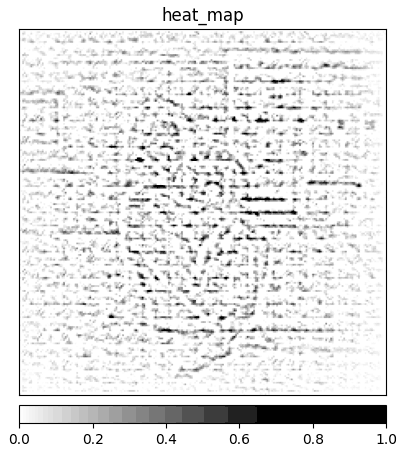
\includegraphics[width=\textwidth]{methods/images/1-4-0-rotation-30-Weimaraner-Weimaraner.png}
    \caption{Deconvolution results}\label{fig:gbp-deconv-attributione}
\end{subfigure}
 \begin{subfigure}{.25\textwidth}
    \centering
    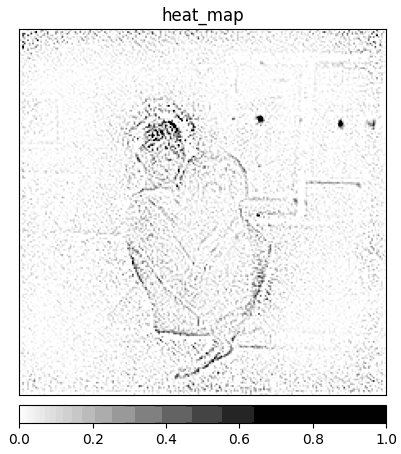
\includegraphics[width=\textwidth]{methods/images/1-4-0-rotation-30-Weimaraner-Weimaraner-gbp.png}
    \caption{GBP results}\label{fig:gbp-gbp-attribution}
\end{subfigure}
 \begin{subfigure}{.25\textwidth}
    \centering
    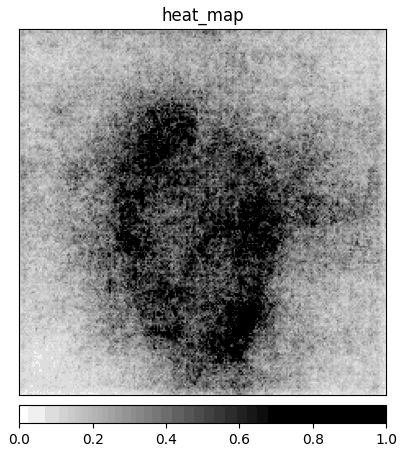
\includegraphics[width=\textwidth]{methods/images/1-4-0-rotation-30-Weimaraner-Weimaraner-saliency.png}
    \caption{Saliency results}\label{fig:gbp-saliency-attribution}
\end{subfigure}

 \caption{Visualisation of saliency maps produced by \textit{Saliency} (\ref{fig:gbp-saliency-attribution}), \textit{Deconvolution} (\ref{fig:gbp-comparision-with-deconv-and-saliency}), and \textit{GBP} (\ref{fig:gbp-gbp-attribution}) of the same input image \ref{fig:gbp-weimaraner} for a class \textit{weimaraner}. All the maps are generated using the same model (ResNet18). Image source: \textit{Stanford Dogs} \cite{stanford-dogs} }\label{fig:gbp-comparision-with-deconv-and-saliency}
\end{figure}

As we can see in Figure \ref{fig:gbp-comparision-with-deconv-and-saliency}, the use of the "guide" significantly reduces the amount of noise generated by the \textit{Saliency} method (Fig. \ref{fig:gbp-saliency-attribution}). The idea of GBP is often misunderstood and interpreted as "applying deconvolution results on the saliency results". This is not true because \textit{ReLU} masking extracted from the deconvnet is applied on every level and therefore affecting the gradient values all the way down to the input of the CNN, not only at the first level of the CNN. 